\documentclass[10pt,a4paper]{article}

\usepackage[a4paper,top=0.85cm,bottom=0.85cm,left=1.05cm,right=1.05cm]{geometry}
\usepackage{fontspec}
\usepackage[french]{babel}
\usepackage[hidelinks]{hyperref}
\usepackage{xcolor}
\usepackage{graphicx}
\usepackage{titlesec}
\usepackage{enumitem}

\setmainfont{Arial}
\pagestyle{empty}
\setlength{\parindent}{0pt}
\setlength{\parskip}{0pt}
\linespread{0.96}
\hyphenpenalty=10000
\exhyphenpenalty=10000
\sloppy
\setlist[itemize]{leftmargin=1.05em,itemsep=0pt,topsep=1pt,parsep=0pt,label=-}
\urlstyle{same}

\definecolor{heading}{HTML}{123867}
\titleformat{\section}{\large\bfseries\color{heading}}{}{0pt}{}[\vspace{-5pt}\rule{\linewidth}{0.5pt}]
\titlespacing{\section}{0pt}{5pt}{3pt}

\newif\ifwithphoto
\withphotofalse
\IfFileExists{with_photo.flag}{\withphototrue}{}

\newcommand{\role}[3]{%
  \textbf{#1} \hfill #3\\
  \textit{#2}\vspace{1pt}
}

\newcommand{\edu}[4]{%
  \textbf{#1} -- #2 \hfill #3 #4\\[-1pt]
}

\begin{document}

\ifwithphoto
\begin{minipage}[c]{0.76\linewidth}
{\LARGE \textbf{Kossi Richard Allado}}\\
\textbf{Étudiant ingénieur en cybersécurité et IA | SOC, DFIR, threat hunting}\\
Beni Mellal, Maroc | +212 621 074 305 | \href{mailto:alladokossirichard2025@gmail.com}{alladokossirichard2025@gmail.com}\\
\href{https://allakori.github.io/}{allakori.github.io} | \href{https://github.com/ALLAKORI}{github.com/ALLAKORI} | \href{https://www.linkedin.com/in/kossi-richard-allado-50177b2a5}{linkedin.com/in/kossi-richard-allado}
\end{minipage}
\hfill
\begin{minipage}[c]{0.18\linewidth}
\raggedleft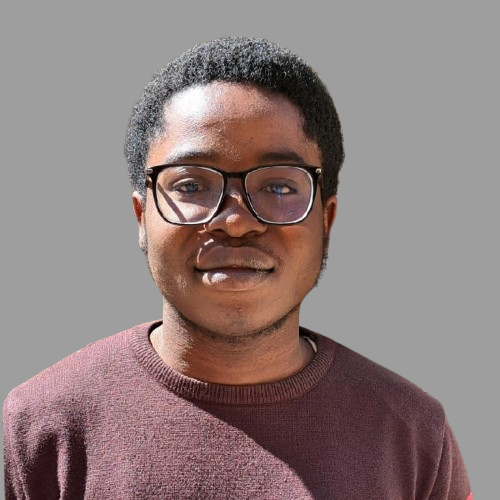
\includegraphics[width=2.35cm]{photo_richard.png}
\end{minipage}
\else
{\LARGE \textbf{Kossi Richard Allado}}\\
\textbf{Étudiant ingénieur en cybersécurité et IA | SOC, DFIR, threat hunting}\\
Beni Mellal, Maroc | +212 621 074 305 | \href{mailto:alladokossirichard2025@gmail.com}{alladokossirichard2025@gmail.com}\\
\href{https://allakori.github.io/}{allakori.github.io} | \href{https://github.com/ALLAKORI}{github.com/ALLAKORI} | \href{https://www.linkedin.com/in/kossi-richard-allado-50177b2a5}{linkedin.com/in/kossi-richard-allado}
\fi

\section{Profil}
Étudiant ingénieur en cybersécurité et IA à l'ENSA Beni Mellal, orienté SOC, DFIR, threat hunting et réponse à incident. Portfolio GitHub structuré autour de labs Linux/DFIR, investigation Splunk, write-ups CTF et documentation technique. Recherche un stage PFA à partir de juillet 2026 en analyse de logs, triage d'alertes, forensic, hardening Linux ou réponse à incident.

\section{Compétences techniques}
\textbf{SOC / détection :} Splunk, Windows logs, Linux logs, auditd, IOC, timeline, MITRE ATT\&CK, alert triage.\\
\textbf{DFIR / forensic :} Volatility, WinPMEM, Autopsy, FTK Imager, artefacts système, connexions réseau, rapport d'incident.\\
\textbf{Systèmes / sécurité :} Linux, SSH, SELinux, AppArmor, Lynis, Keycloak, MFA/TOTP, RBAC, OpenSSL, PKI.\\
\textbf{Automatisation :} Python, Bash, C, SQL, Git/GitHub, Pandas, Scikit-learn, Jupyter.

\section{Projets techniques}
\textbf{Investigation SOC/DFIR d'une intrusion type Volt Typhoon} \hfill 2026\\
\href{https://allakori.github.io/writeups/tryhackme/volt-typhoon/}{allakori.github.io/writeups/tryhackme/volt-typhoon}
\begin{itemize}
  \item Reconstruit une intrusion APT sur 9 phases MITRE ATT\&CK : initial access, execution, persistence, defense evasion, credential access, discovery, lateral movement, collection et C2.
  \item Extrait 10+ indicateurs exploitables : compte compromis, IP source, archive déguisée, web shell, staging directory, C2, Mimikatz URL et journaux effacés.
  \item Produit des requêtes Splunk et une timeline reliant WMIC, PowerShell, certutil, netsh, wevtutil et Mimikatz à l'attaque.
\end{itemize}

\textbf{Linux Security Labs : hardening, audit et forensic} \hfill 2026\\
\href{https://github.com/ALLAKORI/linux-security-labs}{github.com/ALLAKORI/linux-security-labs}
\begin{itemize}
  \item Documenté un workflow Linux couvrant hardening, auditd, détection d'intrusion, acquisition forensic et analyse mémoire.
  \item Corrélé processus, connexions réseau, artefacts système et traces utilisateur dans un rapport orienté remédiation.
\end{itemize}

\textbf{IAM, PKI et sécurisation des accès} \hfill 2025\\
\href{https://github.com/ALLAKORI/cybersecurity-iam-labs}{github.com/ALLAKORI/cybersecurity-iam-labs}
\begin{itemize}
  \item Déployé un laboratoire IAM avec Keycloak : utilisateurs, rôles, MFA/TOTP, RBAC et tests de contrôle d'accès.
  \item Mis en pratique OpenSSL/PKI, SSH hardening et contrôles d'accès pour renforcer la sécurité système.
\end{itemize}

\textbf{CSIA CTF 2026 - 1ère place avec Team GHOSTSHELL} \hfill 2026\\
\href{https://github.com/ALLAKORI/csia-ctf-2026-writeups}{github.com/ALLAKORI/csia-ctf-2026-writeups}
\begin{itemize}
  \item Résolu en équipe des challenges web, OSINT, forensic et stéganographie, puis rédigé des write-ups reproductibles.
\end{itemize}

\section{Expérience}
\role{Stagiaire IA / Maintenance prédictive}{ONEE - Branche Eau, Kasba Tadla}{Août 2025}
\begin{itemize}
  \item Préparé des données capteurs de pompe haute pression et entraîné un modèle Random Forest avec Python, Pandas et Scikit-learn.
  \item Créé une interface Tkinter pour tester les prédictions et présenter un niveau de risque exploitable par l'utilisateur.
\end{itemize}

\section{Formation}
\edu{Cycle ingénieur}{Cybersécurité et Intelligence Artificielle, ENSA Beni Mellal}{2024 - Présent}{}
\edu{DEUST}{Mathématiques, Informatique, Physique, FST Fès}{2022 - 2024}{-- Mention Bien}
\edu{Baccalauréat scientifique}{Série D, Lycée de Djagblé, Togo}{2022}{-- Mention Très Bien}

\section{Certifications et réalisations}
Cisco Ethical Hacker | Google Cybersecurity : Foundations et Play It Safe | TryHackMe Junior Penetration Tester Learning Path | TryHackMe Advent of Cyber 2025 | Udemy Cryptography and Hashing | CSIA CTF 2026 : 1ère place

\section{Langues}
Français : courant | Anglais : professionnel technique | Éwé : langue maternelle

\end{document}
